% !TeX root = ../main.tex

\chapter{基本结构及主要内容}

\section{基本结构}
学位论文包括前置部分、主题部分和结尾部分工三大部分,各部分组成及顺序如图~\ref{fig:sturcture} 所示。

\begin{figure}
\centering
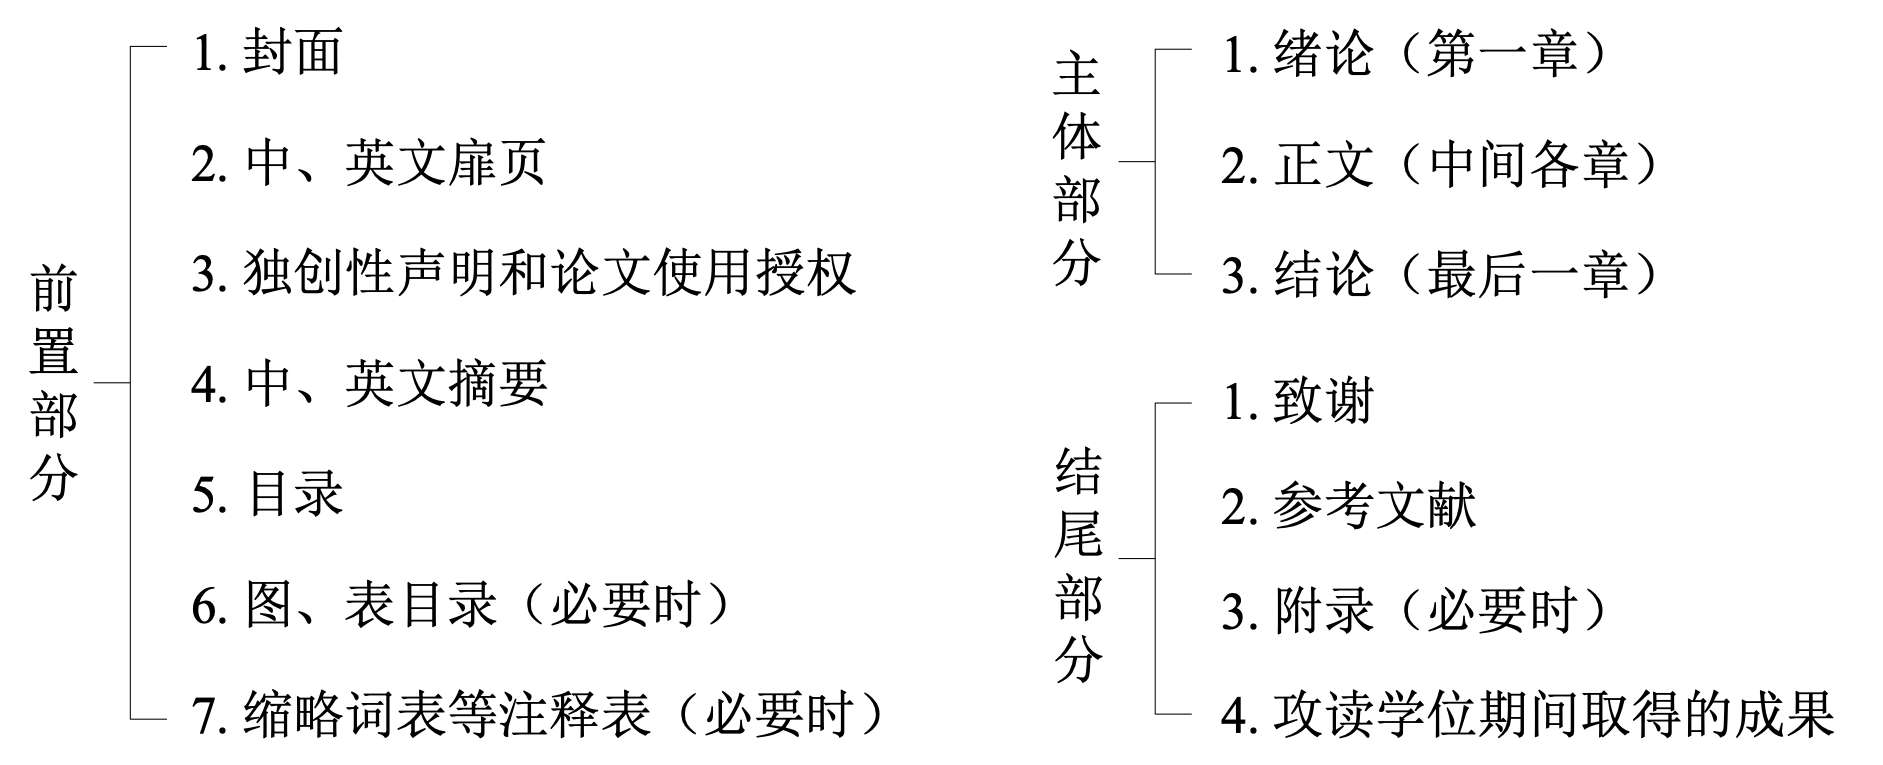
\includegraphics[width=1.0\textwidth]{structure}
\caption{学位论文基本结构}
\label{fig:sturcture}
\end{figure}
\section{前置部分}

\subsection{封面}
内容、样式及填写说明见本文档开头部分。封面由学校文印中心统一制作,不同学位类别对应不同颜色的封面。其中,学术学位博士为墨绿色;专业学位博士为草绿色;学术学位硕士为浅蓝色;专业学位硕士为淡黄色。

论文题目:应以简明的词语反映论文最重要的特定内容,\textbf{避免使用不常用缩略词、字符、代号、公式等},用词须考虑有助于选定关键词和编制题录、文摘等二次文献,可提供检索用的特定实用信息,力求简短,\textbf{一般25字以内}。

学科专业(学术学位)/专业学位类别(专业学位):参照研究生管理信息系统登记的学科专业,以国务院学位委员会批准的学科目录为准。其中,学术学位研究生:按学科目录一级学科培养的,填一级学科;按学校自主设置二级学科培养的,填所属一级学科;按学科目录二级学科培养的,填二级学科。

指导教师:以研究生管理信息系统登记的责任导师为准,且\textbf{只能填写一名指导教师}。若还有其他导师联合指导,可在中、英文扉页相应位置处填写。

\textbf{涉密学位论文},按学校相关规定,还须在封面右上角按“密级★保密期限”格式标注,例如“秘密★10年”。

\subsection{扉页}
内容、样式及填写说明见本文档开头部分。除责任导师外还有其他导师联合指导的,可在本页指导教师位置处填写相关信息。

\subsection{独创性声明和论文使用授权}
内容、样式及填写说明见本文档开头部分。除提交盲审的学位论文外,导师及研究生本人须在独创性声明和论文使用授权相应位置签字。

\subsection{摘要}
摘要是学位论文内容不加注释和评论的简短陈述。摘要应具有独立性和自含性,是一篇简短但意义完整的文章,内容应包括研究目的、研究方法、研究结果和最终结论等,重点是结果和结论,切忌“第一章……第二章……”等论文提纲式陈述。硕士论文中文摘要一般不超过800字,最多不超过1页;博士论文中文摘要一般不超过1500字,最多不超过2页。摘要中不宜使用图、表、公式等。

英文摘要另起一页书写,标题ABSTRACT全部大写,内容与中文摘要一致,翻译准确,博士论文译为“Dissertation”,硕士论文译为“Thesis”,切忌“This paper”。

关键词是用以表示全文主题内容信息的单词或术语。关键词3~5个,与摘要正文之间空一行顶格书写,用逗号隔开。若关键词超过一行,换行后应悬挂缩进对齐。英文关键词应与中文关键词对应,每个单词首字母大写。

摘要和关键词样式见本文档摘要。

\subsection{目录}
目录是论文的提纲。目录内容从“第一章”开始至论文最后一页,包含论文主体部分部分和结尾部分,不包含摘要、缩略词表等前置部分。\footnote{为此,需要将“摘要”等前置部分标题的大纲级别设置为“正文文本”或其他目录不显示的级别,否则目录更新时会自动添加相应标题。}

目录样式见本文档目录。

\subsection{图目录和表目录}
如果论文中使用了大量的图片或表格,可分别列出索引清单置于目录之后。

图、表目录样式见本文档图、表目录。

\subsection{注释表}
如果论文中使用了大量的符号、标志、缩略词、计量单位、自定义名词和术语等,应编写成注释说明汇集表置于目录之后。

符号、缩略词等注释表样式见本文档主要符号表、缩略词表。

\section{主体部分}
\subsection{绪论}
绪论(第一章)应简要阐明论文的选题,选题背景及意义,国内外相关研究成果与进展述评,本论文所要解决的科学与技术问题、所运用的主要理论和方法、基本思路和论文结构等。绪论切忌与摘要雷同或成为摘要的注释。

\subsection{正文}
正文(中间各章)是论文的核心部分,根据学科专业特点和选题情况,可以有不同的写作方式,但应遵循本学科通行的学术规范,必须实事求是,客观真切,准确完备,合乎逻辑,层次分明,简练可读。引用他人研究成果时,应注明出处,不得将其与本人的工作混淆。


学位论文应围绕一个主题,针对某学科领域中的一个具体问题展开深入、系统的研究,并得出有价值的研究结论。论文切忌将几项工作“拼凑”在一起,各章之间应该前后关联,构成一个有机整体。论文各章末尾应有一节“本章小结”,对各章研究内容、方法与成果的简洁准确的总结与概括,也是学位论文最后结论的依据。

\subsection{结论}
结论(最后一章)是论文总体的、最终的结论,而非各章小结的重复,应准确、完整、明确、精练,切忌“第一章……第二章……”等论文提纲式陈述。结论应包括论文的核心观点,重点阐述论文的创造性工作和创新性成果,及其在本领域内的地位、作用和意义,说明论文研究工作的局限或有待进一步研究和探讨的问题,提出未来工作的设想或建议。

结论应严格区分研究生本人的成果与他人的科研工作,常识性的结果或重复他人的结果不应作为结论。在评价自己的研究工作及成果时,要实事求是,除非有足够的证据,否则应避免“首次”、“领先”、“填补空白”等表述。

\section{结尾部分}
\subsection{致谢}
对给予各类资助、指导和协助完成研究工作,以及提供各种对论文工作有利条件的单位及个人表示感谢,一般不超过800字,最多不超过1页。
\subsection{参考文献}
参考文献是文中引用的有具体文字来源的文献集合,按文中引用标注的顺序统一放在致谢之后,具体格式要求见2.10节。
\subsection{附录}
附录是作为论文主体的补充项目(非必须),主要包括正文内不便列出的冗长公式推导、某些重要的原始数据、计算程序及说明等。
\subsection{攻读学位期间取得的成果}
在攻读博士(硕士)学位期间取得的与论文内容相关的研究成果,例如:发表和已录用的学术论文、科研获奖、授权专利等,具体格式要求见2.11节。
\section{各部分标题英文翻译}
用英文撰写的学位论文,内容、格式要求与中文学位论文一致。各部分标题中、英文翻译对照如表\ref{tab:duizhaobiao}所示。

\begin{table}[h]
  \centering
  \caption{学位论文各部分标题中、英文翻译对照表}
  \label{tab:duizhaobiao}
  \begin{tabular}{C{0.45\linewidth}C{0.45\linewidth}}
    \toprule
    中文 & 英文 \\
    \midrule
    摘要 & ABSTRACT  \\
    目录 & Contents \\
    图目录 & Figures \\
    表目录 & Tables \\
    主要符号表 & Symbols \\
    缩略词表 & Acronyms \\
    参考文献 & References \\
    致谢 & Acknowledgements \\
    附录(附录A,附录B)& Appendix (Appendix A, Appendix B) \\
    攻读博士(硕士)学位期间取得的成果 & Research Results Obtained During the Study for Doctoral (Master's) Degree \\
    \bottomrule
  \end{tabular}
\end{table}

% 本模板 \pkg{ustcthesis} 是电子科技大学本科生和研究生学位论文的 \LaTeX{}
% 模板, 按照《\href{https://gradschool.ustc.edu.cn/static/upload/article/picture/ce3b02e5f0274c90b9331ef50ae1ac26.pdf}
% {中国科学技术大学研究生学位论文撰写手册}》(以下简称《撰写手册》)和
% 《\href{https://www.teach.ustc.edu.cn/?attachment_id=13867}
% {中国科学技术大学本科毕业论文(设计)格式}》的要求编写。\footnote{除各章章标题中的数字和字母外,目录中所有内容均不加粗。由于软件限制,本文档目录更新后,可能需要手动对其中的数字章节序号(例如“1.1”“1.1.1”等)取消加粗。}

% Lorem ipsum dolor sit amet, consectetur adipiscing elit, sed do eiusmod tempor
% incididunt ut labore et dolore magna aliqua.
% Ut enim ad minim veniam, quis nostrud exercitation ullamco laboris nisi ut
% aliquip ex ea commodo consequat.
% Duis aute irure dolor in reprehenderit in voluptate velit esse cillum dolore eu
% fugiat nulla pariatur.
% Excepteur sint occaecat cupidatat non proident, sunt in culpa qui officia
% deserunt mollit anim id est laborum.

% \section{脚注}

% Lorem ipsum dolor sit amet, consectetur adipiscing elit, sed do eiusmod tempor
% incididunt ut labore et dolore magna aliqua.
% \footnote{Ut enim ad minim veniam, quis nostrud exercitation ullamco laboris
%   nisi ut aliquip ex ea commodo consequat.
%   Duis aute irure dolor in reprehenderit in voluptate velit esse cillum dolore
%   eu fugiat nulla pariatur.}
